\chapter{\uppercase{Reactor Neutrinos}}

Nuclear reactors are a pure source of electron antineutrinos, $\bar{\nu_e}$, as a result of the fission of isotopes used in the reactor fuel. The first neutrino was discovered using the nuclear reactor at the Savannah River Plant, and reactor sites continue to be popular homes for neutrino detectors. 
In order to perform precision reactor neutrino studies it is important to understand the reactor neutrino flux and spectrum.

\section{Production of Reactor Neutrinos}

Nuclear reactors are powered by the fission of Uranium and Plutonium isotopes in their cores. 
Specifically, in a power reactor, 99.9\% of the power comes from the fission of $^{235}$U, $^{239}$Pu, $^{241}$Pu, and $^{238}$U isotopes. 
The chain reaction begins with a neutron colliding with a nucleus of one of the isotopes. 
This causes the nucleus to split into two fragments, usually of unequal mass, creating an unstable system.
In order to reach stability neutrons have to transform into protons, a process only accomplished through $\beta$ decay, see Figure~\ref{fig:nucchart}.
Each beta decay produces an electron and corresponding electron antineutrino. 
In general a nuclear reactor will produce $\sim 6 \times 10^{20} \bar{\nu_e}$ per GW of thermal energy power \cite{HayesVogel}.

\begin{figure}[h]
	\centering
	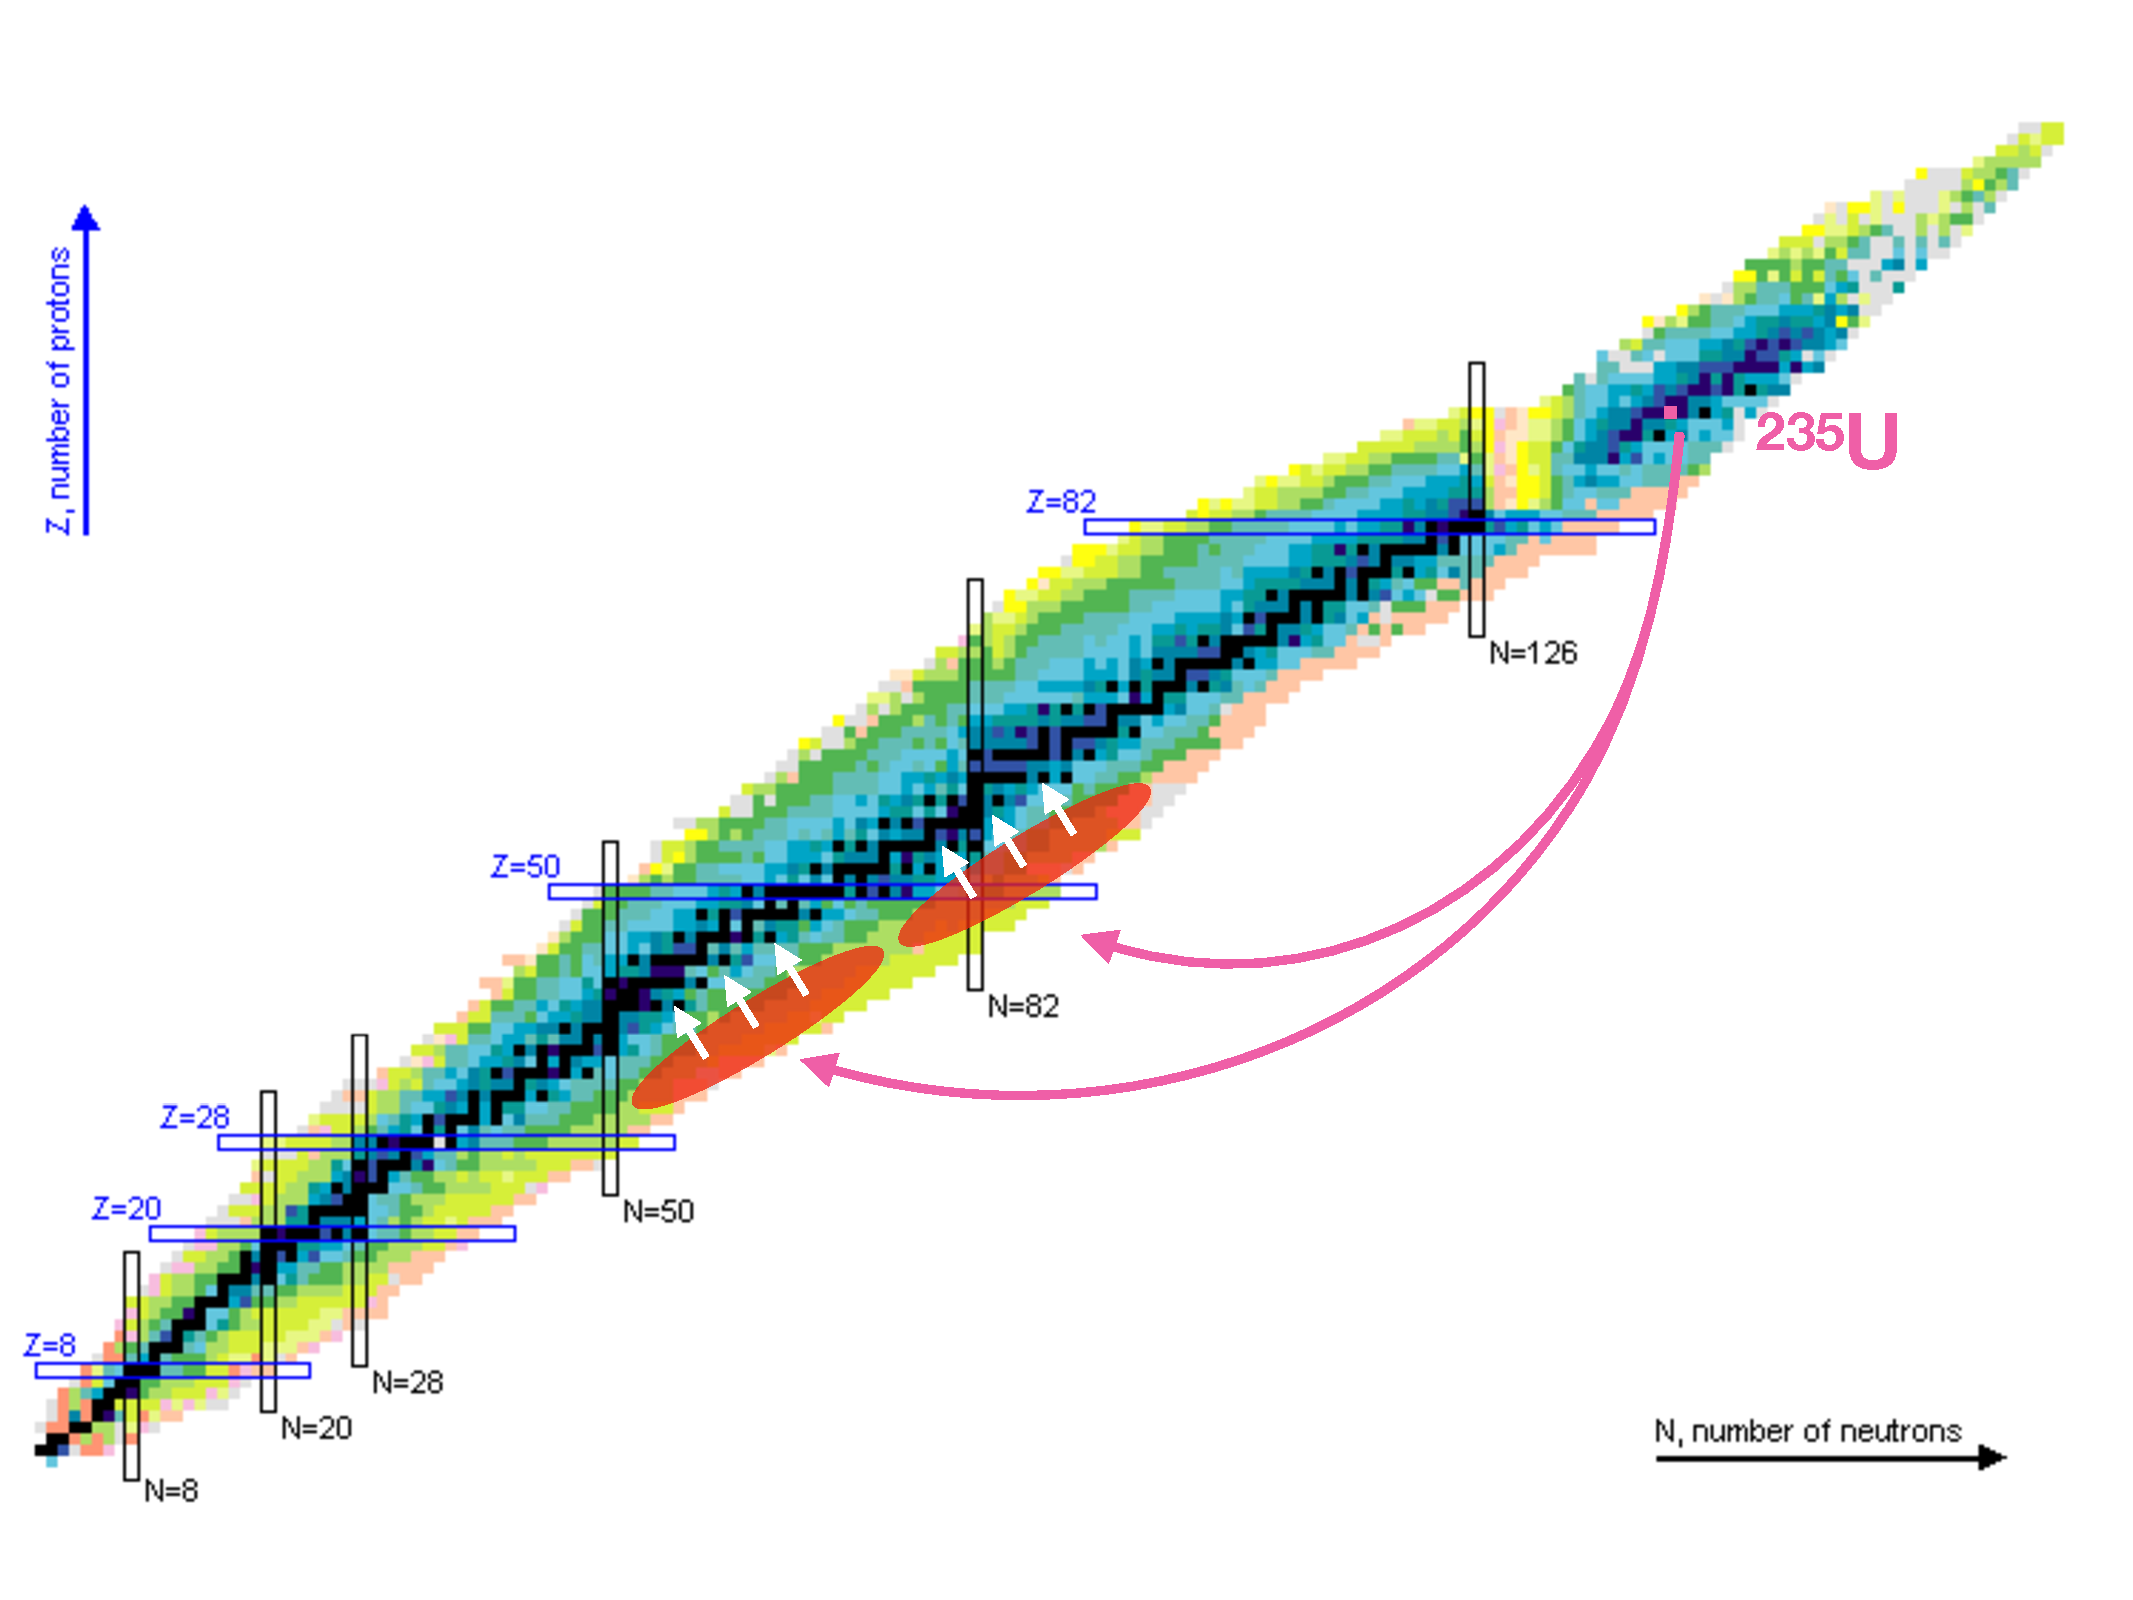
\includegraphics[width=0.75\linewidth]{tex/3-reactorneutrinos-images/NuclideChart_U235}
	\caption{A schematic of the fission of $^{235}$U \cite{NucChart}. After collision with a neutron $^{235}$U will split into two unstable nuclei (pink arrows) which will then $\beta$ decay (white arrows) until stable.}
	\label{fig:nucchart}
\end{figure}


\section{Measuring the Reactor Antineutrino Flux and Spectrum}

The total antineutrino spectrum produced by a nuclear reactor can be expressed as the sum over the spectra for the dominant fissioning isotopes,

\begin{equation}
	S(E_\nu) = \frac{W_{th}}{\sum_{i}(f_i/F)e_i}\sum_{i}\frac{f_i}{F}\left(\frac{dN_i}{dE_\nu}\right) ,
\end{equation}

where $f_i$ is the number of fissions from isotope $i$, $F$ is the total number of fissions, $W_{th}$ is the total reactor thermal energy, $e_i$ is the effective thermal energy per fission contributed by each isotope $i$, and $dN_i/dE_\nu$ is the cumulative $\bar{\nu_e}$ spectrum of $i$ normalized per fission.

There are two methods to determine the $\bar{\nu_e}$ spectrum, \textit{ab initio} summation and electron spectrum conversion.
In the \textit{ab initio} approach the spectrum is determined by summing the contributions of all $\beta$-decay branches of all fission fragments,

\begin{equation}
	\frac{dN_i}{dE_{\bar{\nu}}} =  \sum_{n}Y_n(Z,A,t)\sum_{n,i}b_{n,i}(E^i_0)P_{\bar{\nu}}(E_{\bar{\nu}},E^i_0,Z) ,
\end{equation}

where $Y_n(Z,A,t)$ is the number of $\beta$ decays of the fission fragment $Z, A$ at time $t$, $b_{n,i}(E^i_0)$ are the branching ratios with endpoint energies $E^i_0$, and $P_{\bar{\nu}}(E_{\bar{\nu}},E^i_0,Z)$ is the normalized $\bar{\nu_e}$ spectrum for the branch $n, i$.
The antineutrino spectrum for the four main reactor isotopes calculated using this method can be seen in Figure~\ref{fig:spectrum}. 
Unfortunately, with this method comes several sources of uncertainty. 
The fission yields, $Y_n$ have been determined by a few different groups, but don't always agree and have large uncertainties and not all branching ratios are known. 
For this reason another method can be considered. 

\begin{figure}[t]
	\centering
	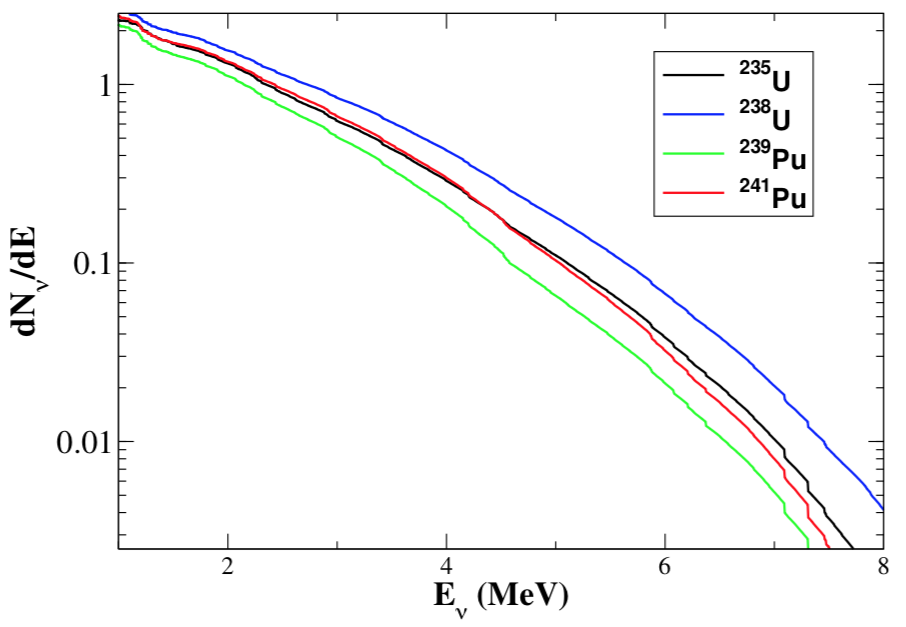
\includegraphics[width=0.7\linewidth]{tex/3-reactorneutrinos-images/Spectrum}
	\caption{The $\bar{\nu_e}$ spectrum predicted by the summation method using the JEFF-3.1.1 database fission fragment yields and the ENDF/B-VII.1 decay library \cite{HayesVogel}.}
	\label{fig:spectrum}
\end{figure}

The electron spectrum conversion method involves converting a measured electron spectrum into an antineutrino spectrum. 
This involves fitting an experimentally defined total beta spectrum with individual beta spectrum  according to their amplitudes, $a_i$, 

\begin{equation}
	\frac{dN_i}{dE_e} = \sum_{i}a_iP(E,E^i_0,Z)
\end{equation}

The conversion to the antineutrino spectrum is then accomplished by replacing the energy $E_e$ in each branch by $E_0 - E_{\bar{\nu}}$, because the electron and the $\bar{\nu_e}$ share the total energy of each $\beta$-decay branch.
The flux per fission is then given as the sum of $\bar{\nu_e}$ spectrum converted from each virtual $\beta$ branch,

\begin{equation}
	\frac{dN_i}{dE_{\bar{\nu}}} = \sum_{i}a_iP(E^i_0-E,E^i_0)
\end{equation}

\todo{New figure?}
\begin{figure}
	\centering
	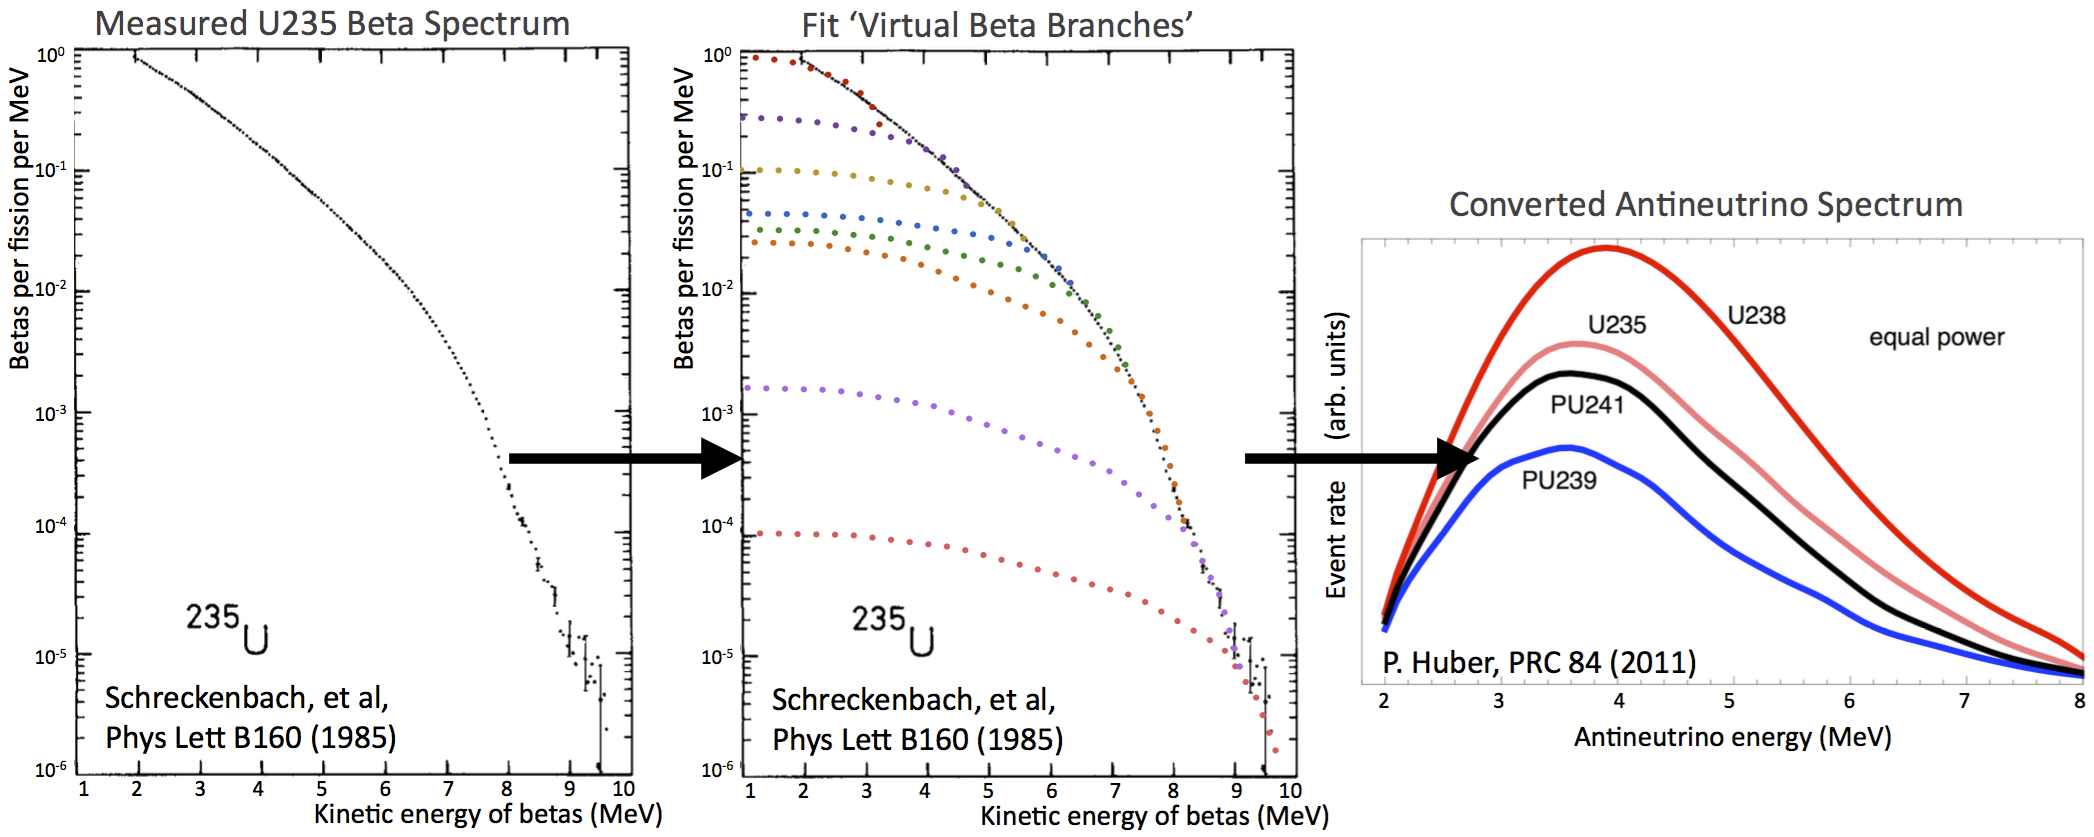
\includegraphics[width=0.7\linewidth]{tex/3-reactorneutrinos-images/betaspecconversion_fixed}
	\caption{}
	\label{fig:betaspecconversionfixed}
\end{figure}




\section{Detection of Reactor Neutrinos}

Though there are several methods that can be used to detect reactor neutrinos, including charge-current ($\bar{\nu_e} + d \rightarrow n + n + e^+$), neutral-current ($\bar{\nu_e} + d \rightarrow n + p + \bar{\nu_e}$), and antineutrino-electron elastic scattering ($\bar{\nu_e} + e^- \rightarrow \bar{\nu_e} + e^-$), the one employed by most experiments is IBD ($\bar{\nu_e} + p \rightarrow e^+ + n$).
The IBD reaction energy threshold is 1.8 MeV and the cross section is relatively high, $\sim 63 \times 10^{-44} \textrm{cm}^2/\textrm{fisson}$ integrated over the entire reactor neutrino energy spectrum \cite{Qian:2018wid}, and can be written as

\begin{equation}
	\sigma^{(0)} \simeq 9.52 \times \left(\frac{E_e^{(0)}p_e^{(0)}}{\textrm{MeV}^2}\right) \times 10^{-44}\textrm{cm}^2
\end{equation}

where $E_e$ and $p_e$ are the energy and momentum of the final-state positron. 

An IBD event is selected by a pair of coincident signals consisting of a positron ionization and annihilation as the prompt signal and a time delayed neutron capture on a proton or nucleus as the delay signal. 
The neutron energy can be backtracked from the prompt signal as
\begin{equation}	
	E_{\bar{\nu}} = E_{prompt} + 0.78~\textrm{MeV} + T_n
\end{equation}
where $T_n$ is the kinetic energy of the recoil neutron which is much smaller than the energy of the neutrino and can therefore be ignored in most cases. 
The IBD cross-section increases with energy, whereas the $\bar{\nu_{e}}$ spectrum decreases with energy creating a detected energy spectrum that peaks around 3.8 MeV and dies off after $\sim$8 MeV, as seen in Figure~\ref{fig:vogel-fig02}. 

In addition to great background rejection and good reconstruction of the neutrino energy, the IBD method of detecting neutrinos also allows the use of liquid scintillators and water as detection mediums. 

\begin{figure}[h]
	\centering
	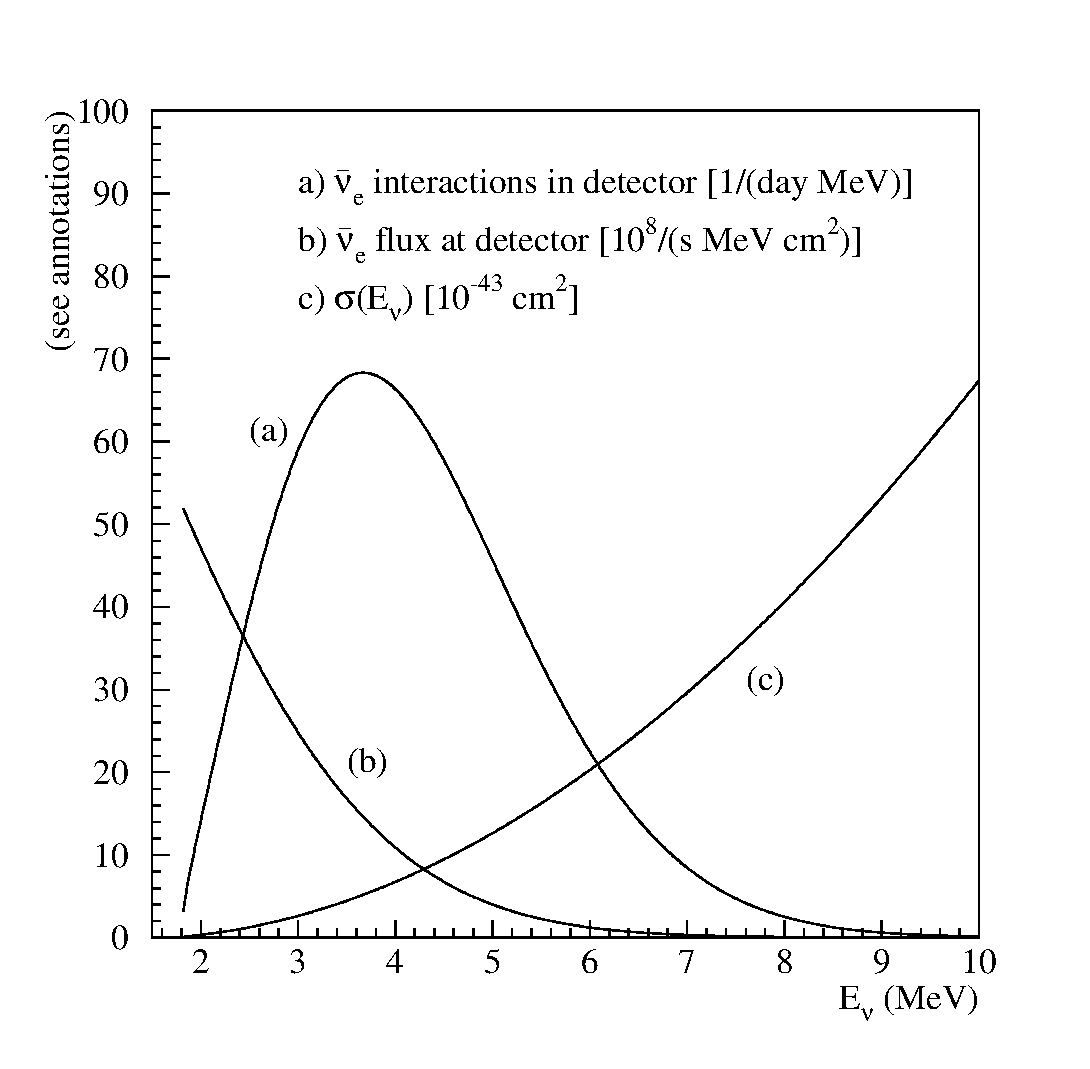
\includegraphics[width=0.7\linewidth]{tex/3-reactorneutrinos-images/vogel-fig02}
	\caption{The IBD spectrum (curve (a)) measured by a 12-ton fiducial mass detector located 0.8 km from a 12-GW$_{th}$ power reactor along with the reactor flux (curve (b)) and IBD cross section (curve (c)) as a function of energy \cite{PDG}.}
	\label{fig:vogel-fig02}
\end{figure}




\section{The Reactor Antineutrino Anomaly}






